\chapter{Cascadas atmosféricas y efecto Cherenkov} \label{EAS_Y_CHERENKOV}
\section{Cascadas atmosféricas} \label{EAS}
	Las cascadas atmosféricas (o EAS por sus siglas en inglés Extensive Air Shower) tienen su origen gracias a la interacción de un CR primario, que llega a la Tierra, con la atmósfera terrestre. La mayor parte de estas EAS son iniciadas por CR con energías mayores a $10^{13}$ eV o $10$ TeV. Cuando estos procesos de colisión son dominados por hadrones se forma lo que conoce como cascada hadrónica, que se propaga en la dirección del momento inicial de la partícula primaria. Luego, muones y neutrinos se forman a partir del decaimiento de piones cargados y kaones, formandose también lo que se conoce como cascada muónica.

	\begin{figure}[h]
		\centering
		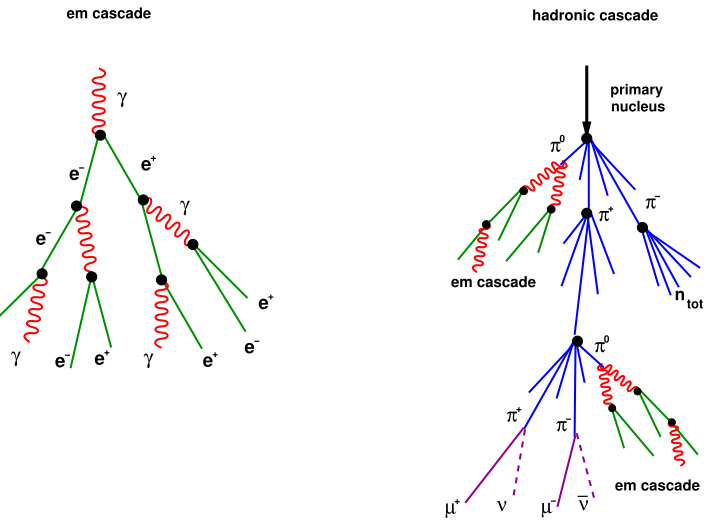
\includegraphics[scale = 0.5]{FIGURAS/CASCADA_LONGITUDINAL.png}
		\caption{Desarrollo longitudinal de una casacada puramente electromagnética y una cascada hadrónica. Los puntos negros representan el lugar de la interacción de la partícula con un núcleo de la atmósfera \cite{MOLLERACH201885}.}
		\label{Cascada_longitudinal}
	\end{figure}

	Los piones neutros y otras partículas decaen en electrones y rayos gamma, formándose así la cascada electromagnética. Aquí se involucran procesos como creación de pares y Bremsstrahlung. De esta manera, una partícula primaria con alta energía puede generar una cascada con gran cantidad de partículas y fotones \cite{GRIEDER2010}.  Dichas cascadas se propagan esencialmente a la velocidad de la luz y pueden alcanzar la superficie terrestre si el CR primario es suficientemenete energético.

	Las cascadas pueden ser iniciadas por hadrones, fotones y electrones, las cascadas iniciadas por fotones o electrones se les conoce como cascadas puramente electromagnéticas. Los fotones de alta energía energía interaccionan con los núcleos de la atmósfera generando la creación de pares $e^+$ y $e^-$, los electrones y positrones interaccionan con los núclos de la atmósfera para porducir fotones mediante Bremsstrahlung \cite{MOLLERACH201885}. A este desarrollo de las cascadas a lo largo de la profundidad atmosférica (medida en gm/cm$^2$) se le conoce como desarrollo longitudinal, la figura \ref{Cascada_longitudinal} nos muestra el desarrollo longitudinal de una cascada puramente electromagnética (inciada por un fotón) y una cascada hadrónica.

\section{Efecto Cherenkov} \label{EFECTO_CHERENKOV}
	Fotones pertenecientes a la radiación visible son producidas cuando una partícula cargada viaja a mayor velocidad que la luz en un medio e interactúa con dicho medio transparente. A esta interacción se conoce como efecto Cherenkov y a los fotones producidos se les conoce como radiación o fotones Cherenkov. La producción de fotones Cherenkov es representado por un frente de onda cónico similar al efecto Doppler, ver figura \ref{Efecto_Cherenkov}, cuyos fotones son emitidos con un ángulo $\theta$ que depende de la velocidad de la partícula y el índice de refreacción del medio, dicha relación se muestra en la ec. \ref{Cherenkov_angulo}. Además, dicho efecto sucederá cuando la velocidad de fase de la partícula, $\beta$, es mayor que el recíproco del índice de refracción del medio, es decir, cuando $\beta > 1/n$, donde $n$ es el índice de refracción del medio \cite{LANNUNZIATA2016547}.
	\begin{equation} \label{Cherenkov_angulo}
		\cos \theta = \frac{1}{\beta n}
	\end{equation}
	
	\begin{figure}[h]
		\centering
		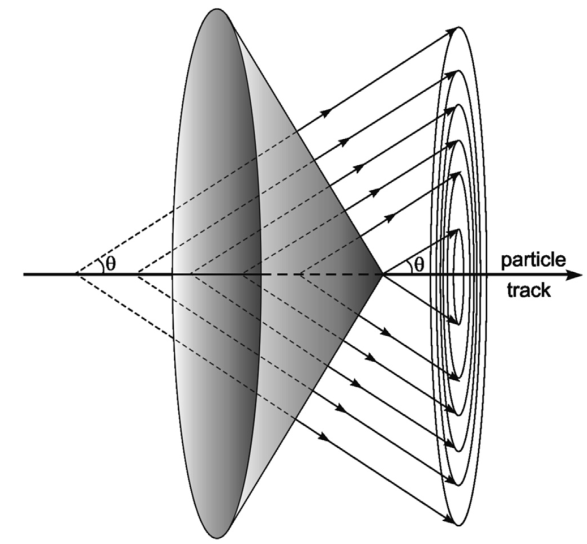
\includegraphics[scale = 0.45]{FIGURAS/EFECTO_CHERENKOV.png}
		\caption{Frente de onda cónico de los fotones producidos por efecto Cherenkov \cite{LANNUNZIATA2016547}.}
		\label{Efecto_Cherenkov}
	\end{figure}